\documentclass{article}
\usepackage{graphicx} % Required for inserting images
\usepackage{tabto}
\usepackage{float}
\usepackage{url}
\usepackage{algpseudocode}
\usepackage{algorithm}
\usepackage{amsmath,amsfonts,amssymb}
\usepackage[backend=biber]{biblatex}
 \addbibresource{references.bib} 

\title{Simplified Metric-Scale 3D Reconstruction of Car Models }
\author{Serban Ionut-Valentin }
\date{November 2024}

\begin{document}

\maketitle



The purpose of this work is to track experiments regarding metric-scale 3D reconstruction, that means given a set of images of an object (in the following experiments the objects are cars) from different point of views/angles, reconstruct the 3D object such that it reflects the metric-scale in real life (the distance between two points in the 3D reconstruction matches the real life distance.)
The following sections show the experiments tried up until now using different machine learning + 3D approaches.
\section{Metric3Dv2 + Mast3R}
\tab Metric3Dv2 \cite{hu2024metric3d} is a foundation model for monocular metric-scale depth trained on 16 million images from 16 datasets of diverse scene types (indoor, outdoor, real and synthetic.) As the benchmarks suggests it achieves rank 3 on NYU Depth and rank 2 on KITTI datasets which proves the reliability of the model in various scenes.\\
\tab \tab Taking this information into consideration, I use this model for predicting the metric-scale depth for each frame in order to create a point cloud. A point cloud is a set of (X, Y, Z) points computed using the formulae (1) and (2).
\begin{equation}
\label{eqn:point_cloud_formula_x}
X = (x - c_x) * Z / f_x 
\end{equation}
\begin{equation}
\label{eqn:point_cloud_formula_y}
Y = (y - c_y) * Z / f_y
\end{equation}\\
\tab \tab Where $(c_x, c_y)$ denote the principal point of the camera (the point on the image plane onto which the perspective center is projected.) and $(f_x, f_y)$ denote the focal length of the camera (angle of view and magnification of a photograph). We suppose these parameters are known in advance and they are correct. The Z value is basically the metric-scale depth value at coordinate $(x, y)$ predicted by Metric3Dv2. Computing these formula for every pixel in the image and we get the point cloud of a single frame (so we project 2D coordinates into 3D.)\\
\tab \tab Having this point cloud, we can assess the accuracy of the metric depth predicted by Metric3Dv2 using the ground truth provided by the dataset. Since the authors have used an Iphone 15 to take the pictures and then used a body scanner for getting the depth, the ground truth is not so accurate and we can test this assumption providing the real dimensions of a car.\\
\tab \tab To provide an example let's take the Figure ~\ref{fig:mock_image}. As you can see it a portrays a Chevrolet Trax from 2013. After searching the specifications of the car on the internet we can conclude that the wheelbase (distance between the wheels) should be around ~2.555 m. \cite{https://www.auto-data.net/en/chevrolet-trax-i-1.6-115hp-17821}. 
\begin{figure}[!ht]
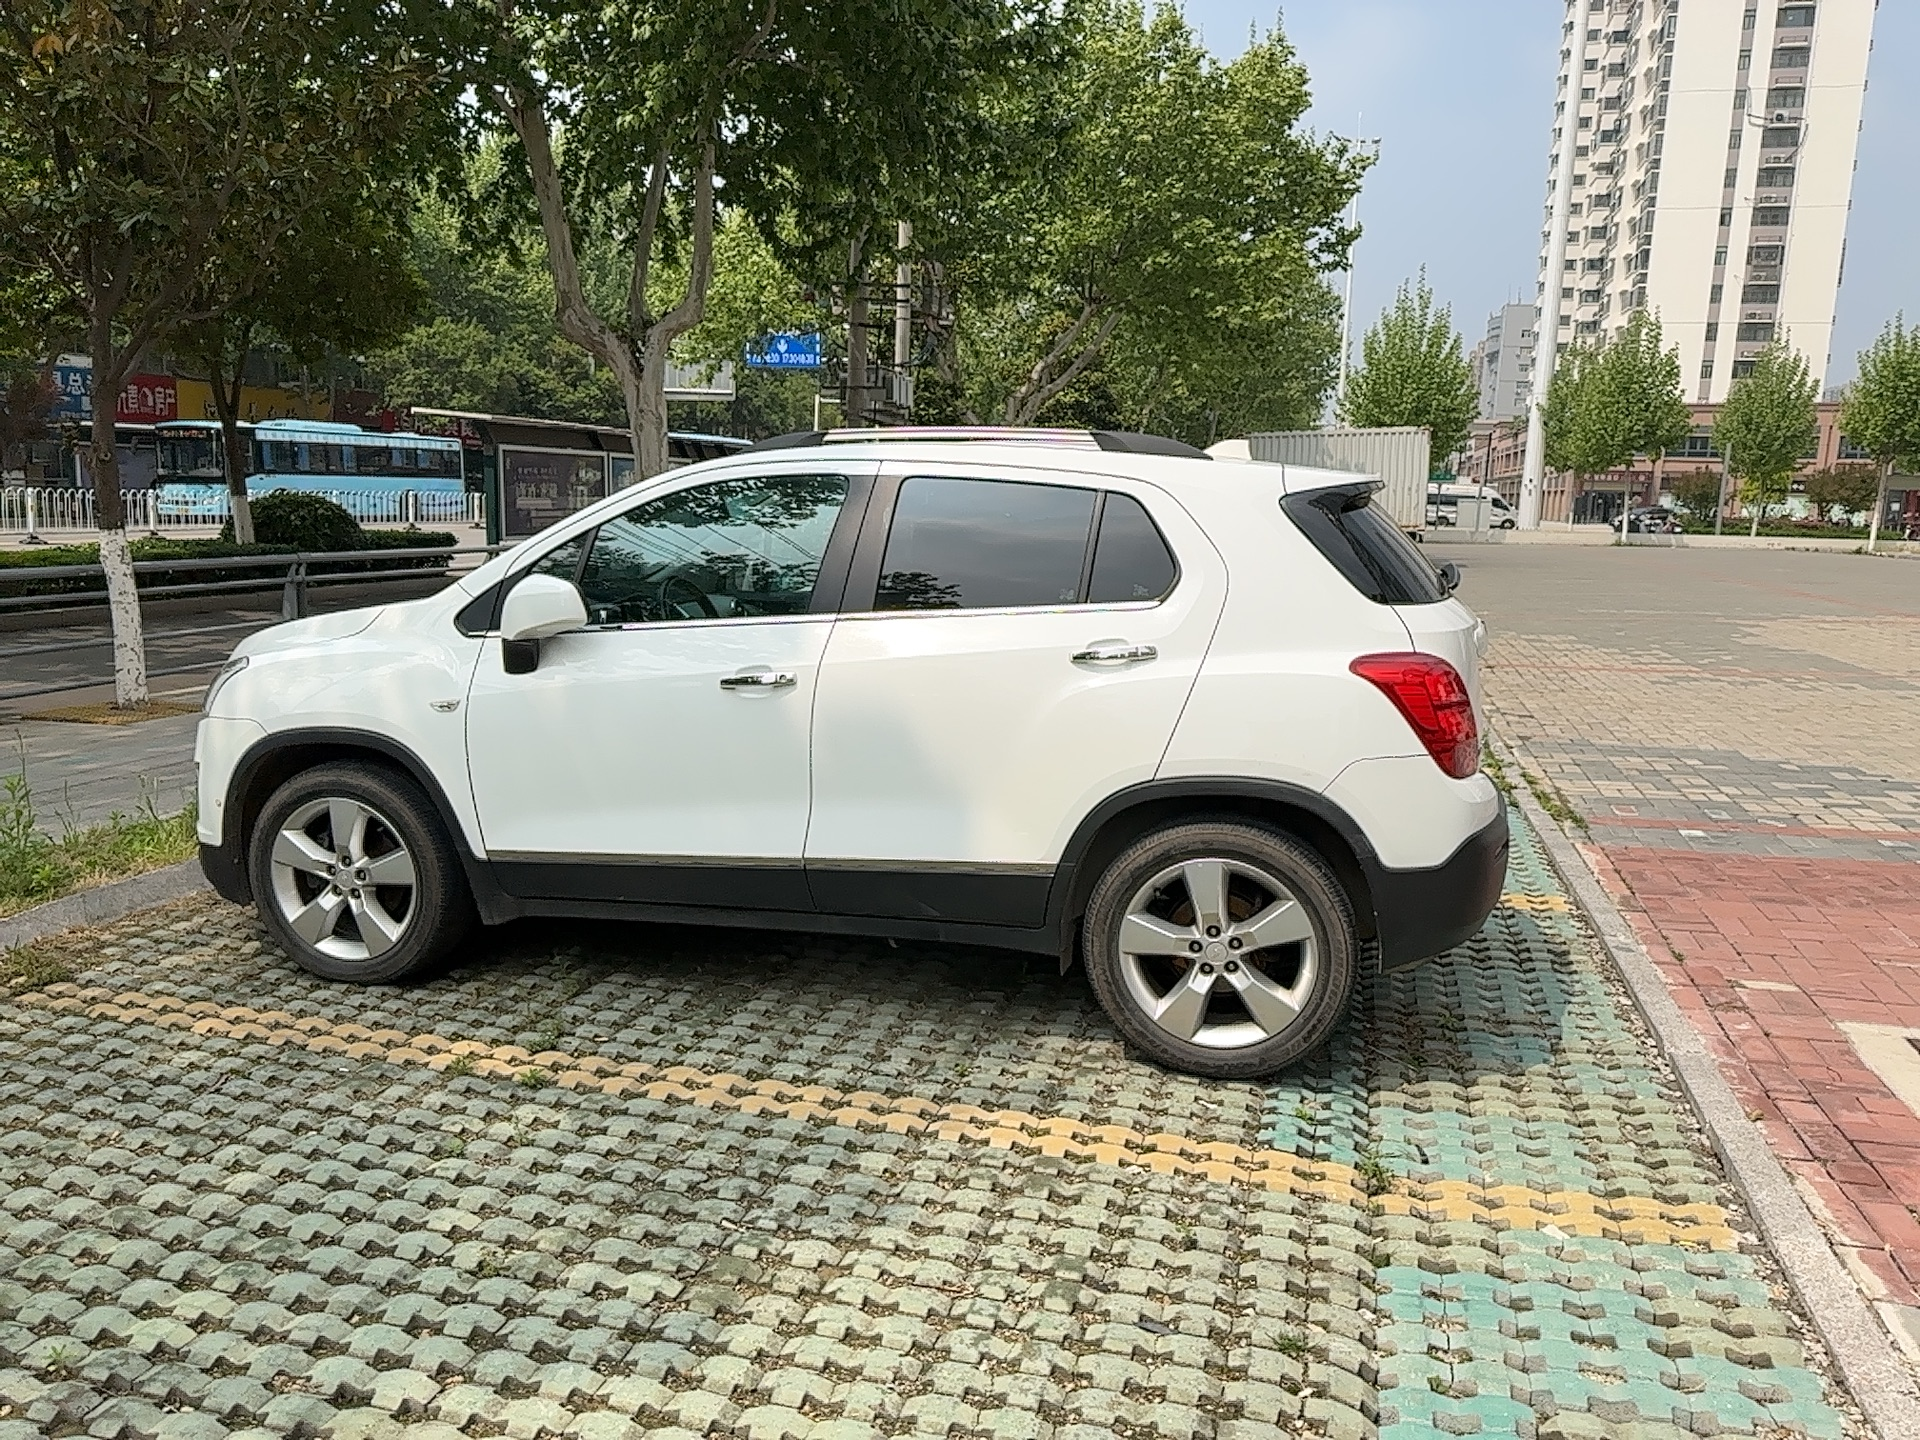
\includegraphics[width=12cm,height=10cm,keepaspectratio]{images/frame_00136.jpg}
\caption{Chevrolet Trax 2013}
\label{fig:mock_image}
\end{figure}\\
\tab \tab Given that the dataset provides the metric depth and also the camera intrinsic parameters we can convert the 2D points (image plane) to 3D points (real world plane) using the aforementioned formulae (1), (2). Plug in the values and we get the following point cloud in Figure ~\ref{fig:point_cloud_gt} on which I also computed the wheelbase. As you can see the ground truth from the dataset is not accurate and as they state in the paper of the dataset \cite{du20243drealcar} it has to be processed using COLMAP (which I didn't manage to install) in order to get more accurate camera parameters.
\begin{figure}[!ht]
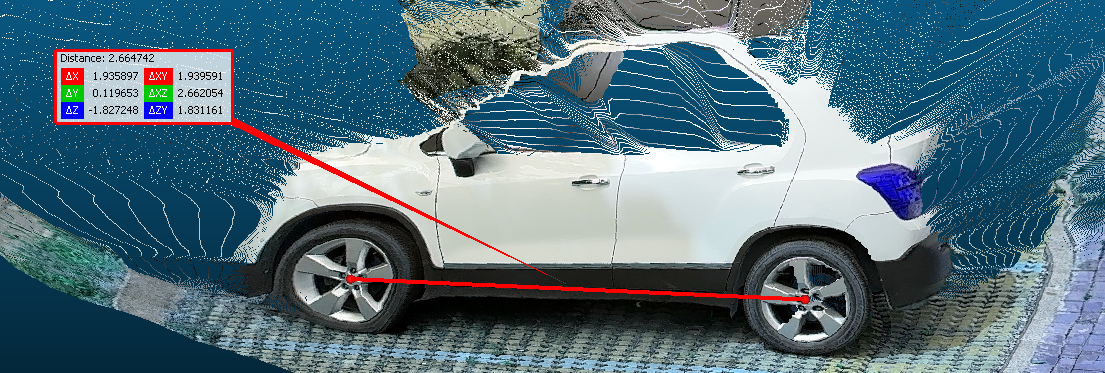
\includegraphics[width=12cm,height=5cm,keepaspectratio]{images/ground_truth_metric_depth.png}
\caption{Ground truth metric depth}
\label{fig:point_cloud_gt}
\end{figure}\\
\tab \tab Running Metric3Dv2 on this image and we get the point cloud in Figure ~\ref{fig:metric_3d_depth}. As you can see the prediction is better than the ground truth depth in the dataset (for Metric3Dv2 we used the same camera intrinsics.) 
\begin{figure}[!ht]
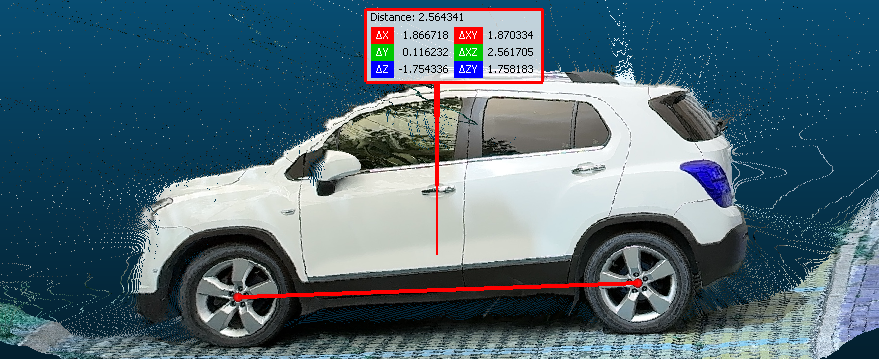
\includegraphics[width=12cm,height=5cm,keepaspectratio]{images/metric3d_depth.png}
\caption{Metric3Dv2 predicted metric depth}
\label{fig:metric_3d_depth}
\end{figure}\\
\tab \tab Unfortunately, since we don't have an accurate metric ground truth to calculate an error (on this particular dataset) we can't state that Metric3Dv2 predicts the depth accurately, so we have to assume that it provides decent results on average, and after the pipeline is completed test this accordingly based on car specifications.\\
\tab \tab Mast3R \cite{mast3r_arxiv24} is a foundation model trained on various datasets that solves a variety of 3D applications such as metric-scale 3D reconstruction, point matching and camera calibration (predicting intrinsic and extrinsic parameters). Since it does all of these 3 (more importantly metric-scale 3D reconstruction which is the problem we want to solve) why not use only Mast3R out of the box in the first place? The problem comes from metric-depth prediction, as you can see in Figure ~\ref{fig:mast3r_prediction} the wheelbase is not even close to the car specifications and the error is over 1 meter, which is not what we want. Basically the main problem with Mast3R is that the predicted metric depth is not accurate (at least out of the box), but the 3D reconstruction (namely the point cloud alignment) is.
\tab \tab Now, since Metric3Dv2 does a good job at metric depth prediction and Mast3R does at 3D reconstruction, why don't we pair these two in order to have an accurate metric-scale 3D one. Now one should state the problem like this: Given a set of images of a car from various camera poses and also the metric-depth associated with them reconstruct the metric-scale car in 3D.\\
\begin{figure}[!ht]
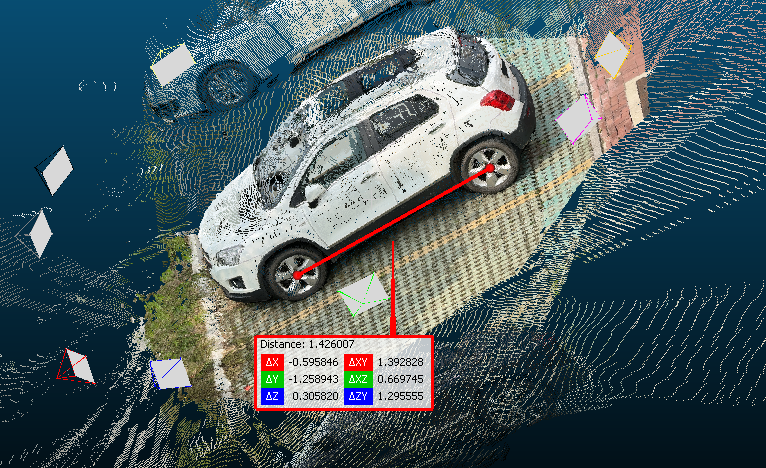
\includegraphics[width=12cm,height=5cm,keepaspectratio]{images/mast3r_pred.png}
\caption{Mast3R predicted metric-scale 3D reconstruction}
\label{fig:mast3r_prediction}
\end{figure}\\
\tab \tab One approach to solve this problem is to use Mast3R for point matching (Figure ~\ref{fig:mast3r_point_matching}) (i.e. given two images, get points from image 1 which correspond with points from image 2), although this one could be solved by using traditional 3D approaches, they do not yield good results especially on flat surfaces such as the a-frame of the car. These points help us translate the point cloud from one frame to the other since we can easily compute using Singular Value Decomposition (SVD) or other traditional machine learning approaches the rotation-translation matrix which minimizes the Mean-Squared Error (i.e. distance between the two sets of points.)
\begin{figure}[!ht]
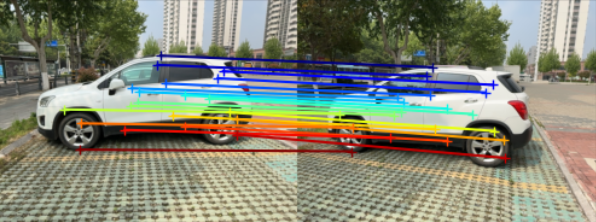
\includegraphics[width=12cm,height=5cm,keepaspectratio]{images/matching_1_2.png}
\caption{Mast3R point matching}
\label{fig:mast3r_point_matching}
\end{figure}\\
\tab \tab So having two 3D point clouds containing matching points (Figure  from different angles (Figure \ref{fig:two_point_clouds}) we can find the rotation-translation matrix in order to go from first point cloud to the second one using the algorithm presented below.\\
\begin{algorithm}
\caption{Algorithm for finding rotation-translation matrix}\label{alg:cap}
\begin{algorithmic}
\State $centroid_1 \gets mean(pcd_1)$
\State $centroid_2 \gets mean(pcd_2)$
\State $normalized_1 \gets pcd_1 - centroid_1$
\State $normalized_2 \gets pcd_2 - centroid_2$
\State $h \gets normalized_1 \cdot {normalized_2}^\intercal$ 
\State $u, s, vt \gets svd(h)$
\State $r \gets {vt}^\intercal \cdot {u}^\intercal$
\State $t \gets -r \cdot centroid_1 + centroid_2$
\State \Return $r, t$
\end{algorithmic}
\end{algorithm}\\
\begin{figure}[!ht]
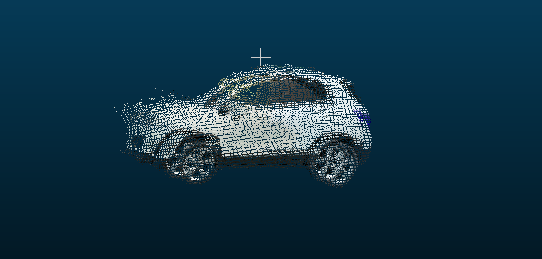
\includegraphics[width=12cm,height=5cm,keepaspectratio]{images/two_point_clouds.png}
\caption{Point clouds from two frames}
\label{fig:two_point_clouds}
\end{figure}\\
\tab \tab After applying this algorithm and concatenating the point clouds we get the following one (Figure \ref{fig:combined_point_cloud}). Since we don't have just two frames (we could have even up to hundreds), we are constrained to combine them all using this approach. Fortunately we can compute the rotation-translation matrices on each 2 consecutive pairs, choose a reference frame (in our case the last one) and by composing the transformations we can go from every frame to the reference frame (e.g. If we have the transformation matrix from frame 1 to frame 2 and the one from frame 2 to frame 3 we can go from frame 1 to frame 3 by the formulae (4) (note that here we use the rotation and translation in the same matrix).\\
\begin{gather}
\label{eqn:composing_rotation}
T_{12} = \begin{bmatrix}
    r_{11} & r_{12} & r_{13} & t_x \\
    r_{21} & r_{22} & r_{23} & t_y \\
    r_{31} & r_{32} & r_{33} & t_z \\
    0 & 0 & 0 & 1
\end{bmatrix} , \quad
T_{23} = \begin{bmatrix}
    r_{11} & r_{12} & r_{13} & t_x \\
    r_{21} & r_{22} & r_{23} & t_y \\
    r_{31} & r_{32} & r_{33} & t_z \\
    0 & 0 & 0 & 1
\end{bmatrix} \\
T_{13} = T_{23} \cdot T_{12}
\end{gather}
\begin{figure}[!ht]
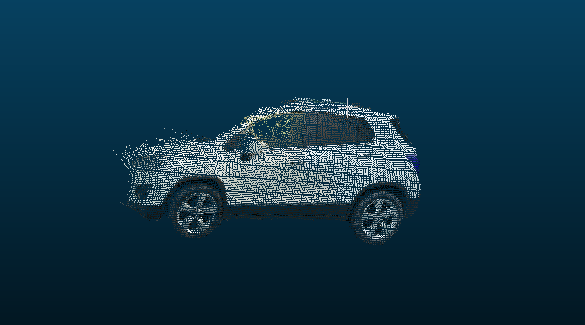
\includegraphics[width=12cm,height=5cm,keepaspectratio]{images/combined_pcd.png}
\caption{Combined point clouds}
\label{fig:combined_point_cloud}
\end{figure}\\
\tab \tab Now, after applying the approach mentioned on roughly 60 frames we get the following point cloud (Figure \ref{fig:final_point_cloud}.) The reconstruction is not accurate especially after getting back to the front of the car from where we previously started, this is because each transformation that we calculate between adjacent frames comes with an error and composing them leads to a greater error so either the composing has to be refined or we have to find another way of aligning the two point clouds. 
\begin{figure}[!ht]
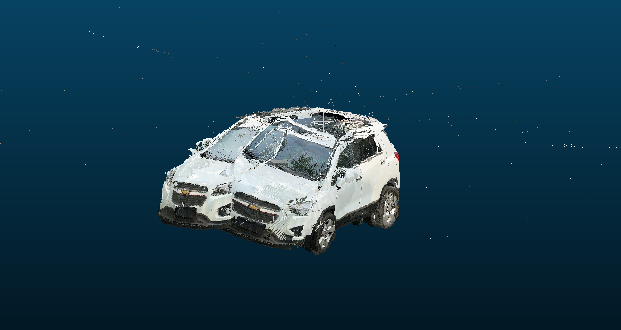
\includegraphics[width=12cm,height=5cm,keepaspectratio]{images/final_pcd_approach_1.png}
\caption{Point cloud after presented approach}
\label{fig:final_point_cloud}
\end{figure}\\
\pagebreak
\printbibliography
\end{document}
